\graphicspath{{img/impl/out}{img/impl}}

\chapter{Implementation}
\label{ch:implementation}
Now that the theoretical foundations of the TASEP and Deep Q-Learning have been introduced, we can start to put the pieces together and implement the smarticles. This chapter will start with the implementation of the classical 2D TASEP to set a baseline for the performance of the smarticles. Then, we will implement the smart TASEP and introduce a number of modifications. 
\\
All code was written in Python to reduce the amount of boilerplate code and to make the code understandable for a wider audience. Python code is often thought to be slow, but the performance-critical parts of the code were outsourced to low-level approaches such as just-in-time compilation and native low-level code used by third-party libraries. 
All code is available at \cite{maertens_smarttasep_github_2023}, with the smart TASEP code being well documented (TODO: and available as pypi package).

\section{Classical 2D TASEP}
\label{sec:implementation-classical-2d-tasep}
The first step is to implement the classical 2D TASEP. This will serve as a baseline for the performance of the smarticles. 
\\
The implementation consists of a simple python script with the main loop for the simulation just-in-time-compiled to machine code using the \texttt{numba} library \cite{lam_numba_2015}. The system is represented as a 2D array of integers, where 0 represents an empty site and 1 represents a site occupied by a particle. The main loop is shown in algorithm \ref{alg:2d-tasep}. In each time step, a random particle is selected and a random direction is chosen. If the target site is empty and the random direction is not backward, the particle moves to the target site and the move counter for the chosen direction is incremented. When different velocities are used, a random number is drawn and the jump is only performed when the random number is smaller than the velocity. In this case, the velocities are floats in the range $(0,1)$ and stored in the array instead of the ones. Finally, the time step counter is incremented and the loop starts again.

\begin{algorithm}[H]
    \caption{Main loop of the 2D TASEP simulation.}
    \label{alg:2d-tasep}
    \begin{algorithmic}
        \State Initialize system $S$ as empty 2D array
        \State Fill in particles randomly (when using velocities, fill in velocities $v\in (0,1)$ instead of ones)
        \State Initialize time step counter $t=0$
        \State Initialize move counters $m_{\text{up}}=0$, $m_{\text{down}}=0$, $m_{\text{right}}=0$
        \While{$t < T$}
            \State Select random position $\bm{x}=(x_1,x_2)^T$ in system
            \If {site $S_{x_1,x_2}\neq 0$}
                \State Select random direction $\bm{d} \in \{\text{up}, \text{down}, \text{right}, \text{left}\}$ with equal probability
                \If {site $\bm{x}+\bm{d}$ == 0 \textbf{and} $\bm{d} \neq \text{left}$ \textbf{and} random $r\in (0,1) < S_{x_1,x_2}$}
                    \State Swap sites $S_{x_1,x_2}$ and $S_{x_1+d_1,x_2+d_2}$ to perform jump
                    \State $m_d \gets m_d + 1$
                \EndIf
            \EndIf
            \State $t \gets t+1$
        \EndWhile
\end{algorithmic}
\end{algorithm}

  
\section{SmartTASEP Python Package}
\subsection{Overview}
\label{subsec:implementation-overview}
The smart TASEP was implemented as a PyPi package available at (TODO). The package is called \texttt{SmartTasep} and can be installed using pip. This makes it easy to not only reproduce the results of this thesis, but also to conduct further research using the smart TASEP. The package is well documented and contains a number of examples that show how to use the package. Features include:
\begin{itemize}
    \item \textbf{Training} of DDQN agents in the 2D TASEP
    \item \textbf{Evaluation} of trained agents
    \begin{itemize}
        \item using \textbf{metrics} such as the particle current
        \item using a \enquote{\textbf{playground}} to test the agent's behavior for custom states
        \item using the \textbf{real-time visualization} of the simulation
    \end{itemize} 
    \item Different \textbf{velocities} for particles
    \item Different \textbf{initial conditions}
    \item Different \textbf{reward structures}
    \item Different \textbf{network architectures}
    \item Different \textbf{replay buffer} implementations (uniform, prioritized)
    \item Different \textbf{hyperparameters}, \textbf{training schedules and environment parameters}
    \item Real-time \textbf{visualization} of the simulation and metrics
    \item \textbf{Saving} and \textbf{loading} of trained agents
\end{itemize}
The package consists of different modules that are shown in figure \ref{fig:implementation}. They will be explained one by one in the following sections. Helper modules and interfaces will not be explained, as they are not relevant for the understanding of the smart TASEP. 

\begin{figure}[h]
    \centering
    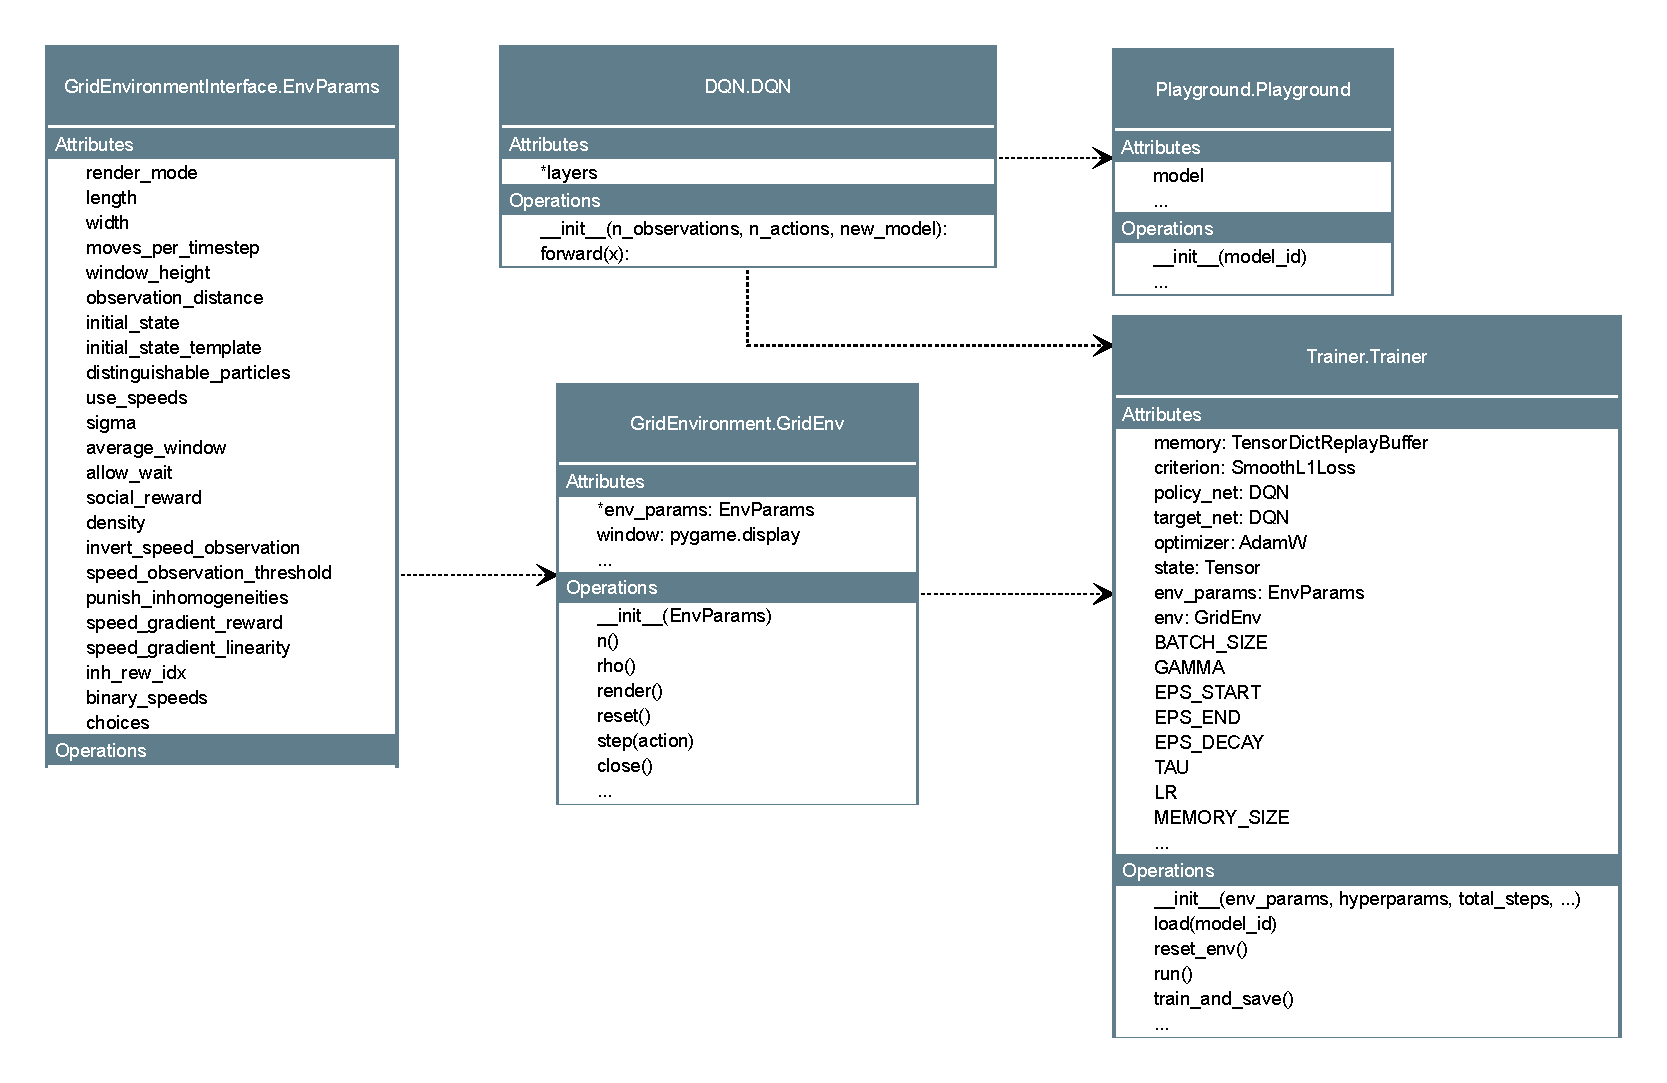
\includegraphics[width=\textwidth]{uml.pdf}
    \caption{UML diagram of the \texttt{SmartTasep} python package. Only selected methods and attributes are shown. The full documentation is available at \cite{maertens_smarttasep_github_2023}.}
    \label{fig:implementation}
\end{figure}


\subsection{GridEnv and EnvParams}
\label{subsec:implementation-gridenv}
The \texttt{GridEnv} class implements the 2D TASEP environment for a reinforcement learning agent. It is a subclass of the \texttt{gym.Env} class from the OpenAI \texttt{gym} library \cite{brockman_openai_2016}. This allows the environment to be used with any reinforcement learning algorithm that is compatible with the OpenAI Gym interface. The environment is initialized with an \texttt{EnvParams} object, which may contain a number of parameters to customize the environment size and initial conditions, the reward structure, the visualization and metrics as well as other properties e.g. to control the dynamics of the reinforcement learning algorithm. 
\\
\\
Internally, the \texttt{GridEnv} class also uses a 2D array to store the state of the system. For indistinguishable particles with equal velocities, this is a binary array, where 0 represents an empty site and 1 represents a site occupied by a particle. Section \ref{subsec:implementation-trainer} will explain that sometimes, particles have to be distinguishable. In that case, the binary array is not suited to store the state. Instead, during initialization, each particle is assigned a unique integer ID, which is stored in the array instead of the ones. If the particles have different velocities, the velocities are stored by adding them to the ID. As the velocities are floats in the range $(0,1)$, they can be stored in the same array without any loss of information. We can retrieve the ID and velocity $v$ of a particle by using the floor and modulo operators on the stored value $s$ respectively:
\begin{equation}
    \text{ID} = \lfloor s \rfloor \text{,} \quad v = s \bmod 1 \text{.}
    \label{eq:state-to-id-velocity}
\end{equation}
This is very memory efficient, as we only need one array to store the state of the system. 
\\
In addition to the state array, the \texttt{GridEnv} also stores the current particle's position in order to be able to calculate the reward after an agent submits its action. 
\\
The following are the two most important methods of the \texttt{GridEnv} class:

\subsubsection{reset}
Resets the environment to its initial state and returns the initial state. Note that in this case, \enquote{state} does not refer to the whole system, but only to the selected particle's observation of the system. 
\\
Agents perceive the system as a $d\times d$ grid centered around them, with the observation distance $d/2$ being a parameter. Observations do not include the particle IDs, as this information is irrelevant to the agent and would even make the problem harder, as the agent would have to learn to distinguish between particles. 
\\
Particle velocities are included in the observations, as they are relevant to the agent. Optionally, the observed velocities can be converted to shifted inverse velocities:
\begin{equation}
    v_{\text{shift, inv}} = 1 - v + v_{\text{shift}} \text{.}
    \label{eq:inverse-velocities}
\end{equation}
This has two possible advantages. Firstly, slow particles are now represented by high values, because they correspond to \enquote{more blockage} in the system. Intuitively, it makes sense to frame the problem in this way, as slow particles are not only worse for the transport, but also more persistent in the observation. Secondly and more importantly, the shift $v_{\text{shift}}$ prevents fast particles from being invisible. Without the velocity inversion, particles with very low velocities become indistinguishable from empty sites, which makes it impossible for the agent to learn to avoid them. The inversion alone does not solve this problem, as particles with very high velocities now become invisible. 
\\
\\
It is important to note that this problem is less about the absolute values of the observations and more about the distinguishability between observations. At first glance, it seems like this rescaling of velocities is not necessary, as the weights can be negative and the biases can be adjusted to compensate for the shifted values. However, this is not the case, as the rescaling is only applied to the particles, not to the empty sites. 


\subsubsection{step}
Takes an action as an argument and returns the next state and the reward after performing the action. Actions are encoded as integers, which, as we will see, correspond to the index of the output neuron with the highest activation. The form of the next state or states depends on the environment parameters. See section \ref{subsubsec:implementation-train} for more details.
\\
\\
The reward is calculated based on the reward structure that was defined in the \texttt{EnvParams} object. Each option can be included or excluded from the reward calculation, which allows for a high degree of customization. Examples include:
\begin{itemize}
    \item The default structure yields a positive reward for moving forward, a negative reward for trying to move into an occupied site and zero reward for waiting or switching lanes. 
    \item The \texttt{social\_reward} option adds a negative reward switching lanes into a site with a particle behind it. The magnitude of the reward is proportional to the velocity of the blocked particle. The analogy in the traffic flow interpretation is the car horn that a driver behind you would use if you switched lanes in front of them.
    \item The \texttt{punish\_inhomogeneties} option combined with the \texttt{inh\_rew\_idx} parameter can add different complex potential-like rewards to encourage the emergence of global structures. This will be explained in more detail in section TODO
\end{itemize}
When rendering is enabled, the step method also renders the state of the system in regular intervals. The system matrix is rendered using the \texttt{pygame} library, which is fast enough to not bottleneck the simulation. Velocities are encoded as colors using the HSL color space, which makes it easy to convert velocities to hues. The velocity range $(0,1)$ is mapped to the hue range $(0,120)$, which corresponds to the red to green range. 



\subsection{DQN}
\label{subsec:implementation-dqn}
The \texttt{DQN} class implements the deep neural network that is used to approximate the action-values $Q(s,a)$. It is a subclass of the \texttt{torch.nn.Module} class from the PyTorch library. The network has two hidden layers and uses the \texttt{ReLU} activation function introduced in section \ref{subsec:activation-functions}. The output layer uses the identity activation function, as we want to approximate the action-values directly. During initialization, the size of the flattened observation array and the number of actions are passed as arguments, to determine the size of the input and output layers respectively. An additional parameter switches between two 128-neuron hidden layers and a 24-neuron hidden layer followed by a 12-neuron hidden layer. 
\\
\\
As a subclass of the \texttt{torch.nn.Module} class, the \texttt{DQN} class implements the \texttt{forward} method, which performs the forward pass. The \texttt{forward} method can be called with a single observation when evaluating the network or with a batch of observations when training the network. Backpropagation is efficiently implemented in PyTorch using automatic differentiation, as explained in section \ref{subsec:backprop}. During a forward pass, all operations (e.g. network layer operations, activation functions, loss function) automatically store the information that is needed for backpropagation in the \texttt{torch.Tensor} objects used for the calculations. When the \texttt{backward} method is called on the loss tensor at the end of the forward pass, the gradients are automatically calculated and stored in the \texttt{grad} attribute of each tensor. These gradients are then used to update the network parameters as will be explained in section \ref{subsec:implementation-trainer}.



\subsection{ReplayBuffer}
\label{subsec:implementation-replaybuffer}
The replay buffer is also one of the performance-critical parts of the implementation. Instead of a naive custom implementation, the \texttt{SmartTasep} package uses the \texttt{TensorDictReplayBuffer} or \texttt{TensorDictPrioritizedReplayBuffer} classes together with the \texttt{LazyTensorStorage} class from the \texttt{torchrl} library \cite{bou_torchrl_2023}. The \texttt{torchrl} library is a reinforcement learning library based on PyTorch that implements many very efficient modules for high performance reinforcement learning training using parallel environments, multithreading and supports computation on the GPU. The \texttt{ReplayBuffer} classes implement very efficient sampling, storage and priority update of single transitions or batches. 
\\
\\
The \texttt{torchrl} library implements many more features that could be used to improve the performance of the smart TASEP, but due to the limited time of this thesis and the early stage of the library, only the replay buffer was used. The \texttt{SmartTasep} package uses the \texttt{TensorDictReplayBuffer} class for uniform sampling and the \texttt{TensorDictPrioritized\-ReplayBuffer} class for prioritized sampling. The \texttt{LazyTensorStorage} class is used internally by these classes to store the transitions. 



\subsection{Trainer}
\label{subsec:implementation-trainer}
The \texttt{Trainer} class is the heart of the \texttt{SmartTasep} package. It implements the training loop and the evaluation loop as well as some additional functionality such as saving and loading trained agents. The following are the most important methods of the \texttt{Trainer} class:

\subsubsection{Constructor}
The constructor method initializes the \texttt{Trainer} object. It takes a number of parameters:
\begin{itemize}
    \item \texttt{env\_params}: An \texttt{EnvParams} object that contains the parameters for the environment as explained in section \ref{subsec:implementation-gridenv}.
    \item \texttt{hyperparams}: A \texttt{Hyperparams} object that contains the hyperparameters for the reinforcement learning algorithm. The structure of the \texttt{Hyperparams} object is the same as the \texttt{EnvParams} object, but the parameters are different.
    \item Additional keyword arguments that control the training schedule, visualization and general algorithm choices such as the replay buffer implementation or whether different networks should be used for the individual particles.
\end{itemize}
After some basic input validation, e.g. checking if any of the parameter choices are incompatible, the constructor method initializes all subcomponents needed for training and evaluation of the agents as well as the visualization in pygame, the plotting in matplotlib and the accumulation of metrics.
\\
A \texttt{GridEnv} object is initialized with the \texttt{EnvParams} object and \texttt{DQN} objects are initialized as Q-networks and policy networks. Depending on the parameter choices, the Q-network and policy network are either shared between all particles or $n$ pairs of separate networks are initialized. In the latter case, the particle velocity range is divided into $n$ equally sized intervals and each pair of networks is responsible for the particles in one of these intervals. This allows different types of particles (e.g. fast, medium and slow for $n=3$) to learn different policies without the space complexity of a separate network for each particle.
\\
The size of the observation arrays and the action space is determined by the \texttt{GridEnv} object and passed to the \texttt{DQN} objects during initialization. The \texttt{ReplayBuffer} objects are initialized with the corresponding parameters from the \texttt{Hyperparams} object. Furthermore, pytorch's \texttt{SmoothL1Loss} loss function is initialized and pytorch's \texttt{AdamW} optimizers (see section \ref{subsec:sgd}) are initialized for each Q-network. 


\subsubsection{train}
\label{subsubsec:implementation-train}
The \texttt{train} method implements the training loop. As the TASEP is not an episodic task, the method consists of only one loop running the simulation for a specified number of time steps. Optionally, the training can be performed pseudo-episodically, where the environment is reset in regular intervals, possibly with changing initial conditions, for example to train smarticles in environments with variable density. I refer to this as \textit{pseudo}-episodic, as we are still using a replay buffer with stored transitions from previous episodes.
\\
\\
Depending on the parameters, the \texttt{train} method uses slightly different algorithms that differ in the way that transitions are stored in the replay buffer. There are essentially three distinct ways to generate transitions:
\begin{enumerate}
    \item \textbf{Immediate transitions:} The environment returns the observation of the particle that took the action immediately after the action was executed. When this observation is used in transitions, the state-next state pairs contain no information about the environment dynamics, as there is no time between the states for the environment/other particles to react to the action. In this case, the smarticles learn a policy for a static environment, while actually living in a very dynamic environment. Note that in this case, the environment has to also return an additional next state for a new particle in order to move different particles in each time step.
    \item \textbf{Weakly correlated transitions:} This is the natural way to combine algorithms \ref{ch:dql} and \ref{alg:2d-tasep}. The environment returns the next observation after picking a new particle which is then used both as the next state stored in the transition and as the current state for the next action. This method only makes sense when the same networks are shared between all particles, as the next state is not the next state of the particle that took the action. Instead, the network learns a policy for an environment where it is thrown around, each new state seemingly random and only weakly correlated with the previous state. This algorithm is used when the \texttt{distinguishable\_particles} parameter is set to \texttt{False}. TODO: Markovian?
    \item \textbf{Delayed transitions:} When particles are distinguishable and the current particle's ID is returned by the environment together with the next state, the next state in a transition can be set to the observation of the same particle that took the action at the time step where the particle is picked again and has to choose its next action. This generates transitions from the reference frame of the particles. A particle is presented a state (observation) $s$, takes an action $a$ and receives an immediate reward $r$ for that action. It then \enquote{sleeps} until it is picked again and receives a new state $s'$. Between these two observations, the environment has changed, as other particles have moved. The transitions now contain additional information, e.g. that slow particles tend to remain stationary while fast particles tend to move forward. This algorithm is used when the \texttt{distinguishable\_particles} parameter is set to \texttt{True}. It requires a temporary storage of the current state and action for each particle for later use when the particle is picked again. A step by step implementation is provided in pseudocode in algorithm \ref{alg:delayed-transitions}.
\end{enumerate}

\begin{algorithm}[h]
    \caption{DQN with delayed transitions and shared networks (difference to algorithm \ref{alg:dqn} highlighted in \textcolor{red}{red})}
    \label{alg:delayed-transitions}
    \begin{algorithmic}
        \State Initialize replay buffer $\mathcal{D}$ to capacity $N$
        \State Initialize Q-network $Q$ with parameters $\theta$
        \State Initialize target network $\hat{Q}$ with parameters $\theta^-=\theta$
        \State Initialize environment to get initial state $s_1$, \textcolor{red}{initial particle ID $i_1$}
        \State Initialize $\epsilon$ to $\epsilon_0$
        \State \textcolor{red}{Initialize temporary storage $\mathcal{M}$ for $(s,a,r)$ tuples indexed by particle ID}
        \For{steps $t=1,\dots,T$}
            \State $\triangleright$ Generate new transition
            \State Perform forward pass through $Q$ to get action-values $Q(s_t, a')$ 
            \State With probability $\epsilon$ select a random action $a_t$, otherwise select $a_t = \arg\!\max_a Q(s_t, a)$
            \State Execute action $a_t$ in environment and observe reward $r_t$, next state $s_{t+1}$ \textcolor{red}{and ID $i_{t+1}$}
            \color{red}
            \State $\mathcal{M}[i_t] \gets (s_t, a_t, r_t)$ 
            \If{$i_{t+1} \in \mathcal{M}$}
                \State Store transition $(^*\mathcal{M}[i_{t+1}], s_{t+1})$ in $\mathcal{D}$
            \EndIf
            \normalcolor
            \State $\triangleright$ Update Q-network parameters
            \State Sample random minibatch of transitions $(\bm{s}, \bm{a}, \bm{r}, \bm{s'})$ from $\mathcal{D}$
            \State Set $\bm{y} = \bm{r} + \gamma \max_{a'} \hat{Q}(\bm{s'}, a')$
            \State Calculate mean loss $\mathcal{L} = \text{mean}(\mathcal{L}(\bm{y}, Q(\bm{s}, \bm{a})))$
            \State \textcolor{red}{Perform optimization (AdamW) of $\theta$ using backpropagation of $\mathcal{L}$}
            \State $\triangleright$ Update target network parameters
            \State Update target network parameters $\theta^- \gets \tau \theta + (1 - \tau) \theta^-$
            \State $\triangleright$ Update exploration rate
            \State Decrease $\epsilon$   
        \EndFor
    \end{algorithmic}
\end{algorithm}
When different speeds and multiple networks are used, algorithm \ref{alg:delayed-transitions} has to be slightly modified. Instead of $Q$, $\hat{Q}$, $\mathcal{D}$, $\mathcal{L}$ and a single AdamW optimizer for $Q$'s parameters $\theta$, we now have an array of $n$ such objects for each of these modules. The correct objects are chosen in each timestep based on the particle's velocity which is extracted from the state. 

\subsubsection{save and load}
The \texttt{save} method all model parameters and collected metrics logs the ID of the newly saved model. The \texttt{load} method loads the model parameters and metrics of a previously saved model. This allows for easy saving and loading of trained agents. When no ID is provided during loading, a table is shown with all available models and their properties. The user can then select a model to load by entering its ID. The \texttt{train\_and\_save} method provides a wrapper for automatically saving the model after training.

\subsubsection{run}
The \texttt{run} method is a stripped down version of the \texttt{train} method that only runs the simulation for a specified number of time steps, omitting all operations only necessary for parameter optimization. A greedy policy is used instead of the epsilon-greedy policy used during training. This method is used for evaluation of trained agents. 


\subsection{Playground}
\label{subsec:implementation-playground}
The \texttt{Playground} class implements a playground for testing the behavior of trained agents. When run, the user chooses a saved model and is presented with a window of two grids of the same size as the model's observation size. The left grid is empty except for the agent in the middle and can be filled by the user. Clicking a grid cell adds or removes an agent and clicking and dragging adds an agent with a velocity proportional to the drag distance. The right grid shows the same state after the agent has taken an action. Figure \ref{fig:playground} shows a screenshot of the playground.

\begin{figure}[h]
    \centering
    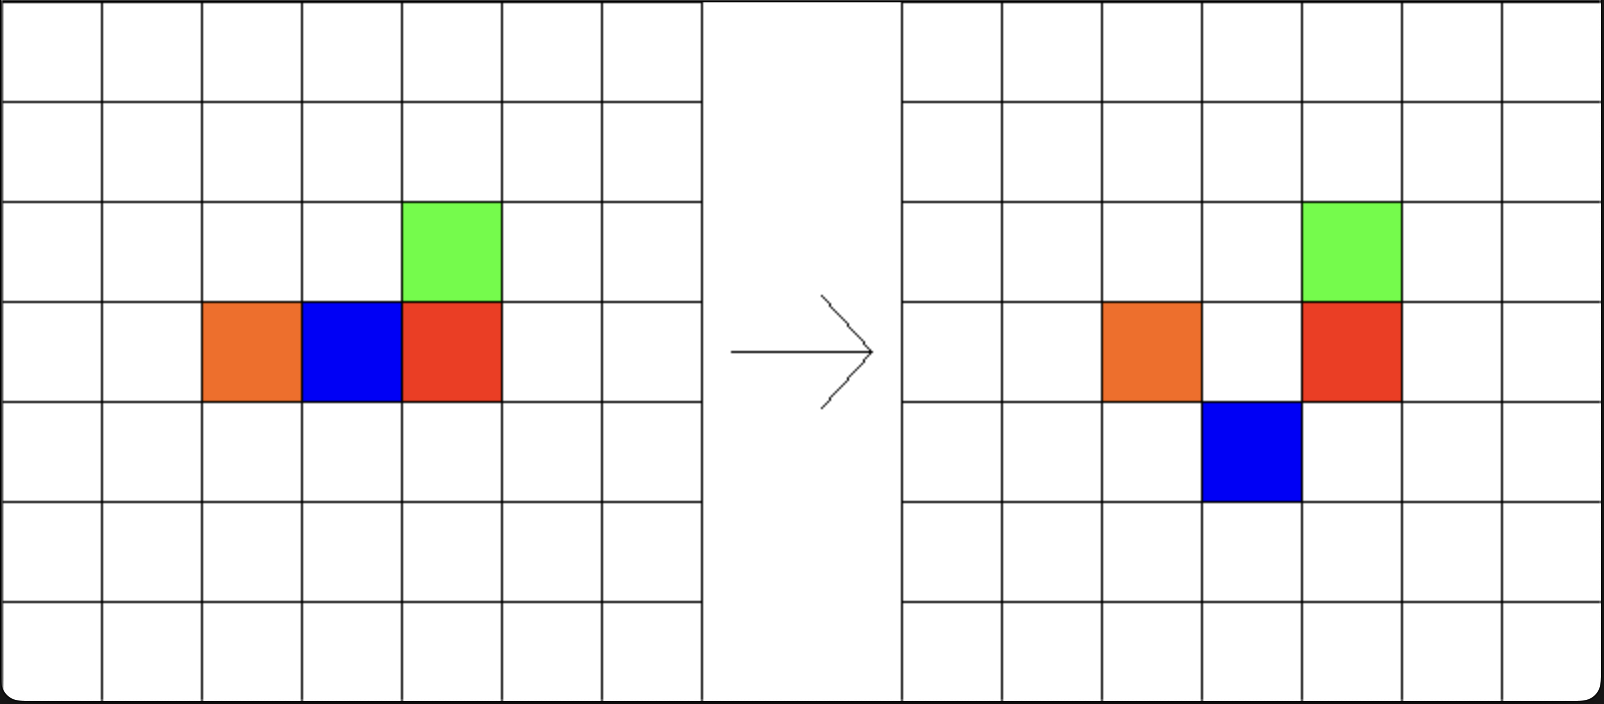
\includegraphics[width=\textwidth]{playground.png}
    \caption{Screenshot of the playground. The state contains one slow particle blocking the agent, a fast particle above the slow one and a particle with average velocity behind the agent. The agent has learned to move around the slow particle in the direction where it's not blocked. More complicated states could be tested e.g. to test the agent's ability to make intelligent decisions based on the speeds and positions of the surrounding particles.}
    \label{fig:playground}
\end{figure}

\section{Hyperparameter Optimization}